\documentclass{article}

% Language setting
% Replace `english' with e.g. `spanish' to change the document language
\usepackage[english]{babel}
\usepackage[BoldFont]{xeCJK}
\usepackage{enumitem}
\usepackage{longtable,booktabs,array}
\usepackage[raggedrightboxes]{ragged2e}
\usepackage{caption} 
%\captionsetup[table]{skip=5pt}
\usepackage{longtable}
\usepackage{makecell}
\usepackage{tablefootnote}
\usepackage{multirow}
\usepackage{multicol}

\usepackage{blindtext} % dummy text, for composition

% Set page size and margins
% Replace `letterpaper' with `a4paper' for UK/EU standard size
\usepackage[a4paper,top=2cm,bottom=2cm,left=2cm,right=2cm,marginparwidth=1.75cm]{geometry}

% Useful packages
\usepackage{amsmath}
\usepackage{amssymb}
\usepackage[table]{xcolor}
\usepackage{graphicx}
\usepackage[colorlinks=true, allcolors=blue]{hyperref}
\usepackage{minted}
\usepackage{listings}
\linespread{1.15}
\setCJKmainfont{cwTeXMing}

\title{\vspace{-1cm}\textbf{Implementation of Intersection Management} \\ \vspace*{0.1cm}\Large\textit{Introduction to Intelligent Vehicles, Final Project}}
\author{標彥廷\,B10902133}
\date{}

\begin{document}

% \begin{titlepage}
%     \centering
%     \vspace*{1cm}
    
%     \Huge
%     \textbf{Implementation of Intersection Management}
    
%     \vspace{0.5cm}
%     \LARGE
%     \textit{Introduction to Intelligent Vehicles, Final Project}
    
%     \vspace{1.5cm}
    
    
%     \text{資工三\,標彥廷\,B10902133}
    
%     \vfill
    
%     \Large
%     Department of Computer Science and Information Engineering\\
%     National Taiwan University\\
%     \today
    
% \end{titlepage}

\maketitle


%\section*{Problem 1}
%\begin{enumerate}[label=(\alph*)]
%    \item Text.
%    \begin{lstlisting}[language=SQL]
% select e.ssn, e.sex, e.salary
 %from employee as e
 %where e.salary <= 30000
% order by e.salary, e.ssn
%    \end{lstlisting}
%    \begin{figure}[H]
%        \centering
%        \includegraphics[width=8cm]{1a.png}
%        \captionof{figure}{}
%    \end{figure}
%    \end{enumerate}

% \inputminted[linenos, bgcolor=bg, breaklines]{cpp}{1.cpp}

\setlength{\columnsep}{0.8cm}
\begin{multicols*}{1}

\begin{abstract}
    This project is an implementation of intersection management. Intersection management is a system that controls the traffic flow in an intersection by scheduling the vehicles to pass the intersection. This project is implemented in Python and visualized by Pygame. I use the graph-based approach with timing conflict graph to simulate the vehicles' movement in the intersection.
    
\end{abstract}
    \section{Introduction} 
    Intersection is the most complex part on roads where traffic flows crisscross, and it is also the place where accidents and conflicts of cars' trajectories are most likely to occur. In a world with each vehicle is autonomous, traditional traffic lights are no longer the best solution for traffic control. Many different approaches have been proposed to solve the intersection management problem. Among the approaches introduced in the lecture, the graph-based approach arroused my interest the most. In this project, I try to simulate the intersection management system using the graph-based approach. I design a road map with a 4-way intersection and assign the vehicles with random starting points and destinations. When the vehicles arrive at the intersection, they will be scheduled to pass the intersection based on the approach mentioned above. The project is implemented in Python and visualized by Pygame. The source codes are available at \url{https://github.com/yenting-biao/Intersection-Management}.

    \section{Preliminary}
    \subsection{Conflict Zone}
    A conflict zone is a region in the intersection where the trajectories of two vehicles intersect. If we do not schedule the vehicles to pass the intersection properly, the vehicles in the conflict zone may collide with each other. Therefore, it is not allowed to have two vehicles in the conflict zone at the same time.
    \subsection{Timing Conflict Graph}
    Timing conflict graph is a directed graph that represents the conflict relationship between the vehicles. Each node in the graph represents a vehicle and a conflict zone, and the edges represent the conflict relationship between the vehicles. There are three types of edges in the timing conflict graph:
    \begin{itemize}[itemsep=0pt, leftmargin=*]
        \item \textbf{Type-1 edges}: The same vehicle's trajectory. An edge from node $(i,j)$ to node $(i,k)$ means that the vehicle $i$ is must pass conflict zone $j$ first and then conflict zone $k$.
        \item \textbf{Type-2 edges}: The conflict of trajectories of different vehicles from the same lane. An edge from node $(i,j)$ to node $(k,j)$ means that vehicle $i$ and vehicle $k$ are from the same lane and vehicle $k$ is preceding vehicle $i$, but both vehicles need to pass the conflict zone $j$. Therefore, vehicle $i$ must pass the conflict zone $j$ first and then vehicle $k$ can pass the conflict zone $j$.
        \item \textbf{Type-3 edges}: The conflict of trajectories of different vehicles from different lanes. An edge from node $(i,j)$ to node $(k,j)$ and another edge from node $(k,j)$ to node $(i,j)$ mean that vehicle $i$ and vehicle $k$ are from different lanes but both vehicles need to pass the conflict zone $j$, and thus we need to resolve this conflict.
    \end{itemize}
    
    When solving the intersection management problem with timing conflict graph, we need to remove some type-3 edges to resolve the conflict. To be more specific, for each pair of node (i, j) and (k, j), if there are type 3 edges from both (i, j) to (k, j) and  (k, j) to (i, j), then we should remove exactly one of them. Note that we should preserve all the type-1 and type-2 edges in the timing conflict graph because they are the necessary conditions for the vehicles to pass the intersection. However, in general scenario, an acyclic timing conflict graph obtained by removing some type-3 edges may not be a feasible solution. Deadlocks may still occur. Therefore, we need to verify the acyclic timing conflict graph by constructing a resource conflict graph.
    
    \subsection{Graph-Based Verification}
    Resource conflict graph is a directed converted from timing conflict graph. It represent the source relationship. I will not list the full rule of the conversion here. The key idea is that if there is an edge from node (i, j) to node (i, k) and another edge from node (i, k) to node (i, l) in the timing conflict graph, the resouce conflict graph would be an edge from node (i, j, k) to node (i, k, l). If the resouce conflict graph is acyclic, then the solution of the timing conflict graph is feasible. Otherwise, we need to try another removval of type-3 edges in the timing conflict graph and re-verify the acyclic timing conflict graph.

    \section{Formulation}
    In my implementation, the intersection is a square with 5 by 5 grids. For simplicity, each grid is a conflict zone, so there are 25 conflict zones in the intersection. An example of the map and cars' states is shown in Figure \ref{fig:map}. The vehicles is represented as a dot, with their sources and destinations randomly assigned. The seed in the codes is fixed, so the results can be reproduced. I use a coordinate system to keep track of the vehicles' positions. Before a vehicle arrives at the intersection, it can just go ahead if there is no other vehicle right in front of it. When a vehicle is about to enter the intersection, the control center will schedule the vehicle to pass the intersection based on the timing conflict graph, and then the vehicle can continue to move to its destination.
    \begin{figure}[H]
        \centering
        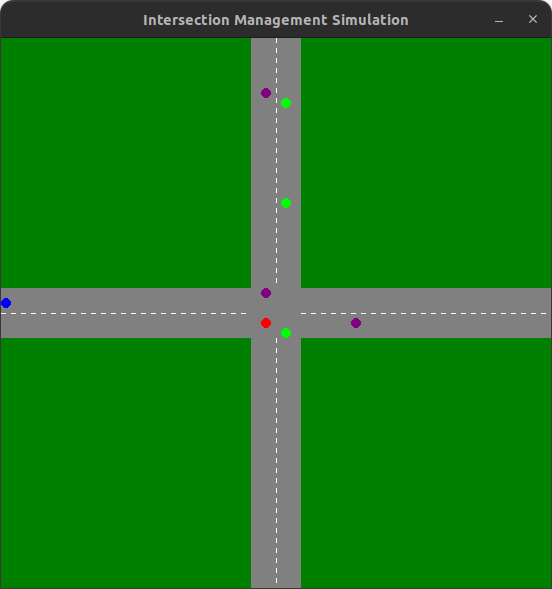
\includegraphics[width=0.4\textwidth]{images/map.png}
        \caption{An example of the map and cars' states}
        \label{fig:map}
    \end{figure}

    \section{Proposed Approach and Implementation Results}
    Here I will introduce the key parts of how I solve the intersection management problem in my implementation. In every time step, the control center will check if there are vehicles about to enter the intersection in the next step. If there are, the control center will add these vehicles to the timing conflict graph and try to resolve the conflicts. The Python code I wrote to build the timing conflict graph is shown in Listing \ref{lst:build-timing-conflict-graph} in Appendix. Note that the control center in my implementation is a class. You may notice that in my implementation, there does not exist type-2 edges in the timing conflict graph as I only schedule the vehicles that are about to enter the conflict zone in the next time step. This is because after some consideration, I found that if there are consecutive cars from the same lane, it is quite difficult to determine how many of them should be added into the schedule, and when to add them in. Therefore, for simplicity, the control center I implemented would not schedule the vehicles until they are about to enter the intersection. Although the throughput of the intersection may be lower than the optimal solution, the vehicles can still pass the intersection without colliding with each other. In real world scenario, it is important that the vehicles can pass the intersection safely, and the control center I implemented can achieve this goal.
    
    Now, let us talk about the details about how the control center schedule the cars based on the timing conflict graph just built. According to what I have mentioned in the preliminary section, we need to remove some type-3 edges in the timing conflict graph to resolve the conflicts. The Python code I wrote to remove the cycles in the timing conflict graph is shown in Listing \ref{lst:cycle-removal} in Appendix. The function \texttt{removeCycle} will enumerate all the possible combinations of edge removal on each pair of nodes that have type-3 edges. For each combination, it will check whether this graph is acyclic. If it is acyclic, then it will return true as it is a feasible solution. Originally, it should build resource conflict graph and verify the acyclic timing conflict graph. However, as the timing conflict graph has only type-1 and type-3 edges, I skip the resource conflict graph construction and verification in my implementation. It can be shown that this would not cause colliding of vehicles in the intersection. Finally, we can use the adjacency list of the acyclic timing conflict graph to schedule the vehicles to pass the intersection. The vehicles will be scheduled to pass the intersection in topological order of the adjacency list. To see the demo video of the implementation, please visit \url{https://youtu.be/fz_0AevhWUs}.

    

    \section{Conclusion}
    In this project, I implement a simplified version of intersection management system using the graph-based approach. The vehicles are scheduled to pass the intersection based on the timing conflict graph without colliding with each other. However, the throughput of the intersection can be improved. Besides, the road map in real world is more complex and the vehicles can have more sophisticated behaviors, which is also another point that can be improved in my implementation.

    \section*{Statement}
    The report does not have any double assignment or any completed work before this semester.

    \section*{References}
    \begin{itemize}[itemsep=0pt, leftmargin=*]
        \item Lecture 6 Slides of Introduction to Intelligent Vehicles, by Prof. Chung-Wei Lin
        \item Github Copilot for coding
    \end{itemize}
\end{multicols*}

\newpage
\section*{Appendix}

\begin{listing}[H]
    \begin{minted}[
        breaklines,
        frame=lines,
        framesep=2mm,
        baselinestretch=1.2,
        fontsize=\footnotesize,
    ]{python}
def constructTimingConflictGraph(self):
self.nodes = {}
self.edges: list[tuple[int, int, int]] = []  # directed edges (src, dst, type)
conflictCars = {}
for car in self.carList:
    for i in range(len(car["trajectory"])):
        self.nodes[(car["index"], car["trajectory"][i])] = len(self.nodes)
        if car["trajectory"][i] not in conflictCars:
            conflictCars[car["trajectory"][i]] = [car["index"]]
        else:
            conflictCars[car["trajectory"][i]].append(car["index"])
        if i > 0:
            self.edges.append(
                (
                    self.nodes[(car["index"], car["trajectory"][i - 1])],
                    self.nodes[(car["index"], car["trajectory"][i])],
                    1,  # Type 1 edge
                )
            )
for key, value in conflictCars.items():
    if len(value) > 1:
        for i in range(len(value)):
            for j in range(i + 1, len(value)):
                self.edges.append(
                    (
                        self.nodes[(value[i], key)],
                        self.nodes[(value[j], key)],
                        3,  # Type 3 edge
                    )
                )
                self.edges.append(
                    (
                        self.nodes[(value[j], key)],
                        self.nodes[(value[i], key)],
                        3,  # Type 3 edge
                    )
                )
    \end{minted}
    \caption{Build the timing conflict graph}
    \label{lst:build-timing-conflict-graph}
\end{listing}

\begin{listing}[H]
    \begin{minted}[
        breaklines,
        frame=lines,
        framesep=2mm,
        baselinestretch=1.2,
        fontsize=\footnotesize,
    ]{python}
def removeCycle(self):
type1Edges = [
    (self.edges[i][0], self.edges[i][1])
    for i in range(len(self.edges))
    if self.edges[i][2] == 1
]
type3Edges = [
    (self.edges[i][0], self.edges[i][1])
    for i in range(len(self.edges))
    if self.edges[i][2] == 3 and self.edges[i][0] < self.edges[i][1]
]
# We only choose one type3 edges for each pair as we will enumerate all possible combinations

def enumerateCombinations(ind: int) -> list[list[int]]:
    if ind == len(type3Edges):
        return [[]]

    laterComb = enumerateCombinations(ind + 1)
    result = []
    for comb in laterComb:
        result.append([(type3Edges[ind][0], type3Edges[ind][1])] + comb)
        result.append([(type3Edges[ind][1], type3Edges[ind][0])] + comb)
    return result

adjList = {}
for edge in type1Edges:
    if edge[0] not in adjList:
        adjList[edge[0]] = [edge[1]]
    else:
        adjList[edge[0]].append(edge[1])

enumerateResult = enumerateCombinations(0)
# print("enumerateResult: ", enumerateResult)
for enum in enumerateResult:
    tmpAdjList = adjList.copy()
    for edge in enum:
        if edge[0] not in tmpAdjList:
            tmpAdjList[edge[0]] = [edge[1]]
        else:
            tmpAdjList[edge[0]].append(edge[1])
    if self._isAcyclic(0, tmpAdjList):
        self.adjList = tmpAdjList
        # print("AdjList: ", self.adjList)
        if self.isValid():
            return True  # self.adjList
return None
    \end{minted}
    \caption{Cycle Removal in Timing Conflict Graph}
    \label{lst:cycle-removal}
\end{listing}

\end{document}